\documentclass[12pt, a4paper]{article}

% Required Packages
\usepackage[utf8]{inputenc}
\usepackage{graphicx}
\usepackage{geometry}
\usepackage{fancyhdr}
\usepackage{hyperref}
\usepackage{subcaption}
\usepackage{float}
\usepackage{amsmath}
\usepackage{booktabs}

% Page Geometry
\geometry{top=1in, bottom=1in, left=1in, right=1in}

% Set the graphics path to the subfolder where images are placed
\graphicspath{{Images/}}

% Header and Footer Setup
\pagestyle{fancy}
\fancyhf{}
\rhead{Microcontroller-Based Overcurrent Relay}
\lhead{Abd El-Rahman Muhammad Saad 19017058}
\cfoot{\thepage}

% Hyperlink Setup
\hypersetup{
	colorlinks=true,
	linkcolor=blue,
	filecolor=magenta,      
	urlcolor=blue,
}

\begin{document}
	
	% ---------------- TITLE PAGE ---------------- %
	\begin{titlepage}
		\begin{flushleft}
			\begin{minipage}{0.15\textwidth}
				
\includegraphics[width=\textwidth]{logo.png} 
			\end{minipage}%
			\hspace{0.3cm}
			\begin{minipage}{0.7\textwidth}
				{\scshape\large Alexandria University} \\[0.1cm]
				{\scshape\normalsize Faculty of Engineering} \\[0.1cm]
				{\scshape\normalsize Electrical Engineering Department}
			\end{minipage}
		\end{flushleft}
		
		\vspace{2.0cm}
		\centering
		{\Huge\bfseries Power System Protection \par}
		\vspace{0.4cm}
		{\Large\bfseries Microcontroller-Based Overcurrent Relay Implementation: Very Inverse Time Characteristic \par}
		
		\vspace{1.0cm}
		{\Large\itshape Prepared by:\par}
		\vspace{0.2cm}
		{\Large \textbf{Abd El-Rahman Muhammad Saad Muhammad}\par}
		{\large \textbf{ID:} 19017058\par}
		
		\vfill
		{\large \textbf{Project Repository Link:}\par}
		{\normalsize \href{https://github.com/Abd-El-Rhman-Saad/Overcurrent-Relay-with-Very-Inverse-Type.git}{Click here to access the Code and Details on GitHub}}\par
		
		\vfill
		{\large \textbf{Date:} May 2026 \par}
	\end{titlepage}
	
	\newpage
	
	\begin{abstract}
		This report details the design and hardware implementation of a microcontroller-based digital overcurrent relay conforming to the IEC Very Inverse time-current characteristic. Overcurrent relays are critical components in power system protection, designed to isolate faults while coordinating with other protective devices. Using an Arduino Uno as the core processing unit, the system continuously monitors the load current via a ZMCT103C/PZEM current sensor. If the measured current exceeds the pre-set pickup value ($I_s$), the microcontroller calculates the exact tripping time based on the Time Multiplier Setting (TMS) and initiates a trip signal to a relay module. The project integrates an I2C LCD for real-time monitoring, push buttons for parameter adjustment, and a buzzer for fault annunciation. The implemented system demonstrates the feasibility and accuracy of using embedded systems for dynamic, inverse-time power system protection.
	\end{abstract}
	
	\newpage
	\tableofcontents
	\newpage
	
	% ---------------- SECTION 1: INTRODUCTION ---------------- %
	\section{Introduction and Theoretical Background}
	Overcurrent protection is the most widely used form of protection in radial distribution systems. An overcurrent relay operates when the load current exceeds a predefined threshold (Pickup Current, $I_s$). To achieve selectivity and proper coordination between primary and backup relays, Inverse Definite Minimum Time (IDMT) characteristics are utilized.
	
	This project implements the \textbf{IEC Very Inverse} characteristic, which provides a steeper curve compared to standard inverse relays, making it highly suitable for applications where the fault current magnitude drops rapidly as the distance from the source increases.
	
	The operating time ($t$) for an IEC Very Inverse relay is governed by the following standardized equation:
	\begin{equation}
		t = \frac{13.5}{\left(\frac{I}{I_s}\right) - 1} \times TMS
	\end{equation}
	Where:
	\begin{itemize}
		\item $t$: Operating (tripping) time in seconds.
		\item $I$: Actual measured fault current.
		\item $I_s$: Pickup current setting.
		\item $TMS$: Time Multiplier Setting, used to shift the curve vertically for coordination.
	\end{itemize}
	
	\newpage
	% ---------------- SECTION 2: HARDWARE COMPONENTS ---------------- %
	\section{Hardware System Components}
	The prototype was built using highly reliable, commercially available embedded components to form a complete data acquisition, processing, and tripping loop.
	
	\begin{figure}[H]
		\centering
		\begin{subfigure}{0.3\textwidth}
			\centering
			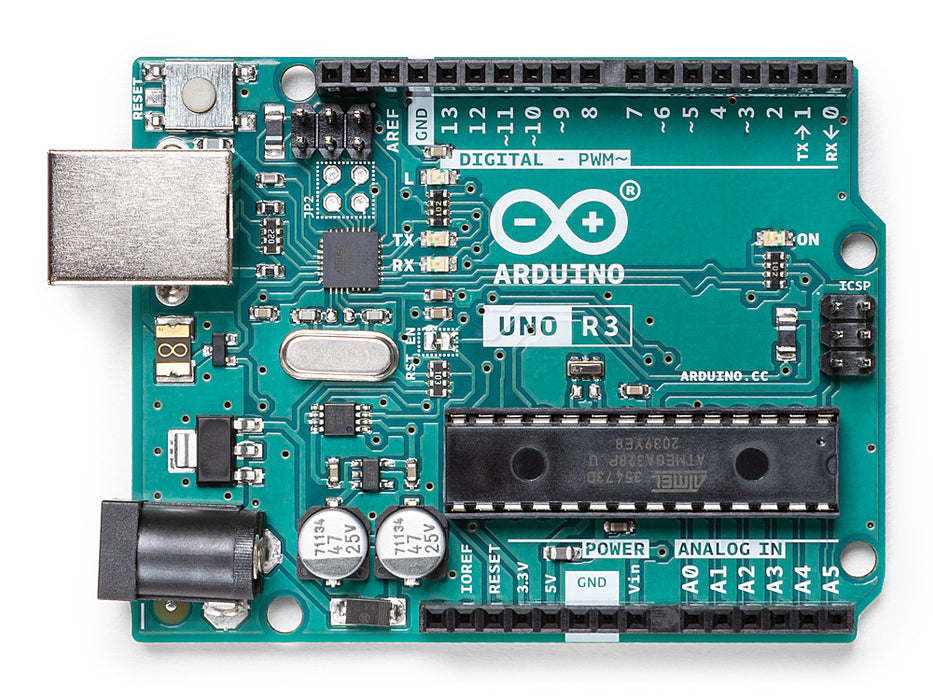
\includegraphics[width=0.8\textwidth]{Arduino.jpg}
			\caption{Arduino Uno}
		\end{subfigure}
		\hfill
		\begin{subfigure}{0.3\textwidth}
			\centering
			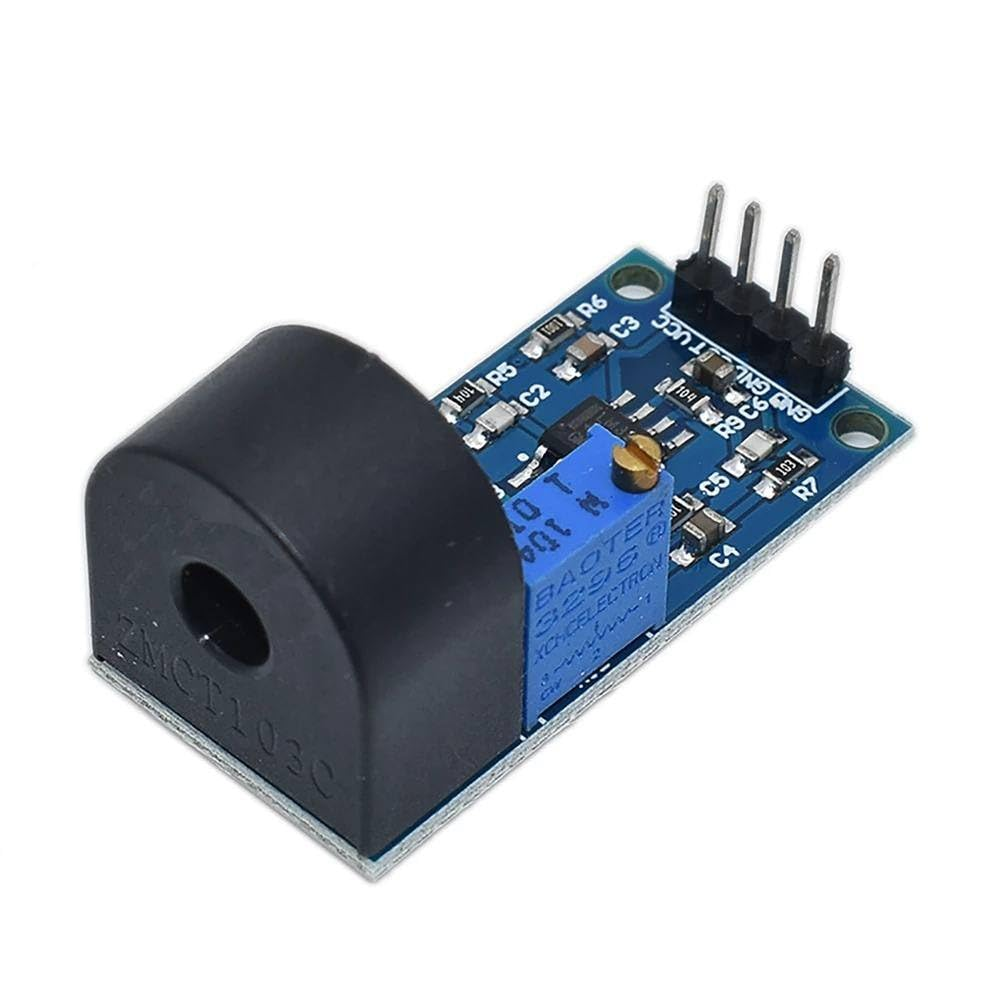
\includegraphics[width=0.8\textwidth]{ZMCT103C.jpg}
			\caption{ZMCT103C Sensor}
		\end{subfigure}
		\hfill
		\begin{subfigure}{0.3\textwidth}
			\centering
			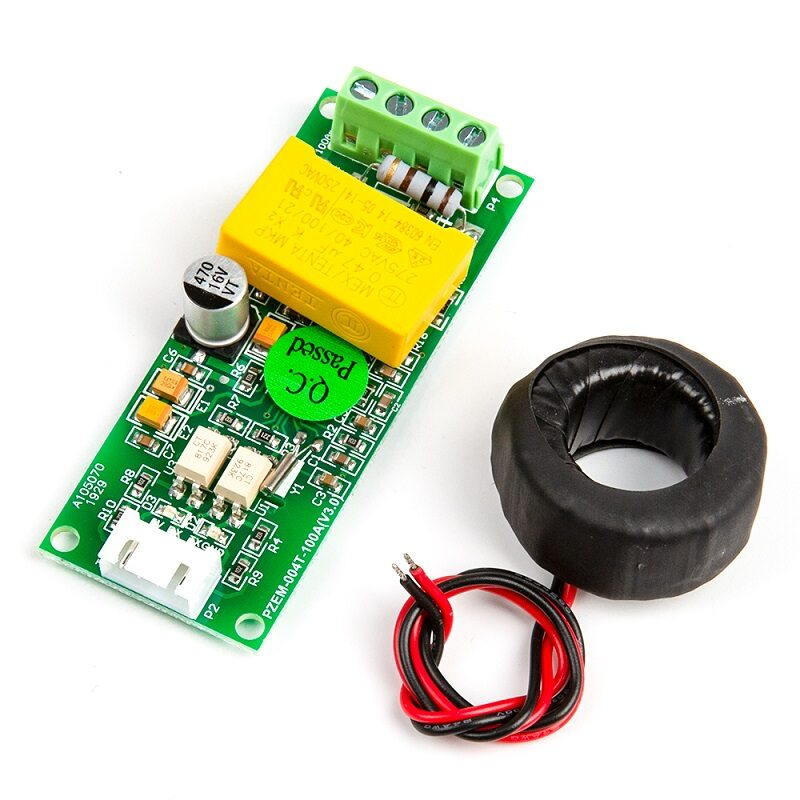
\includegraphics[width=0.8\textwidth]{PZEM.jpg}
			\caption{PZEM-004T}
		\end{subfigure}
		
		\vspace{0.5cm}
		\begin{subfigure}{0.3\textwidth}
			\centering
			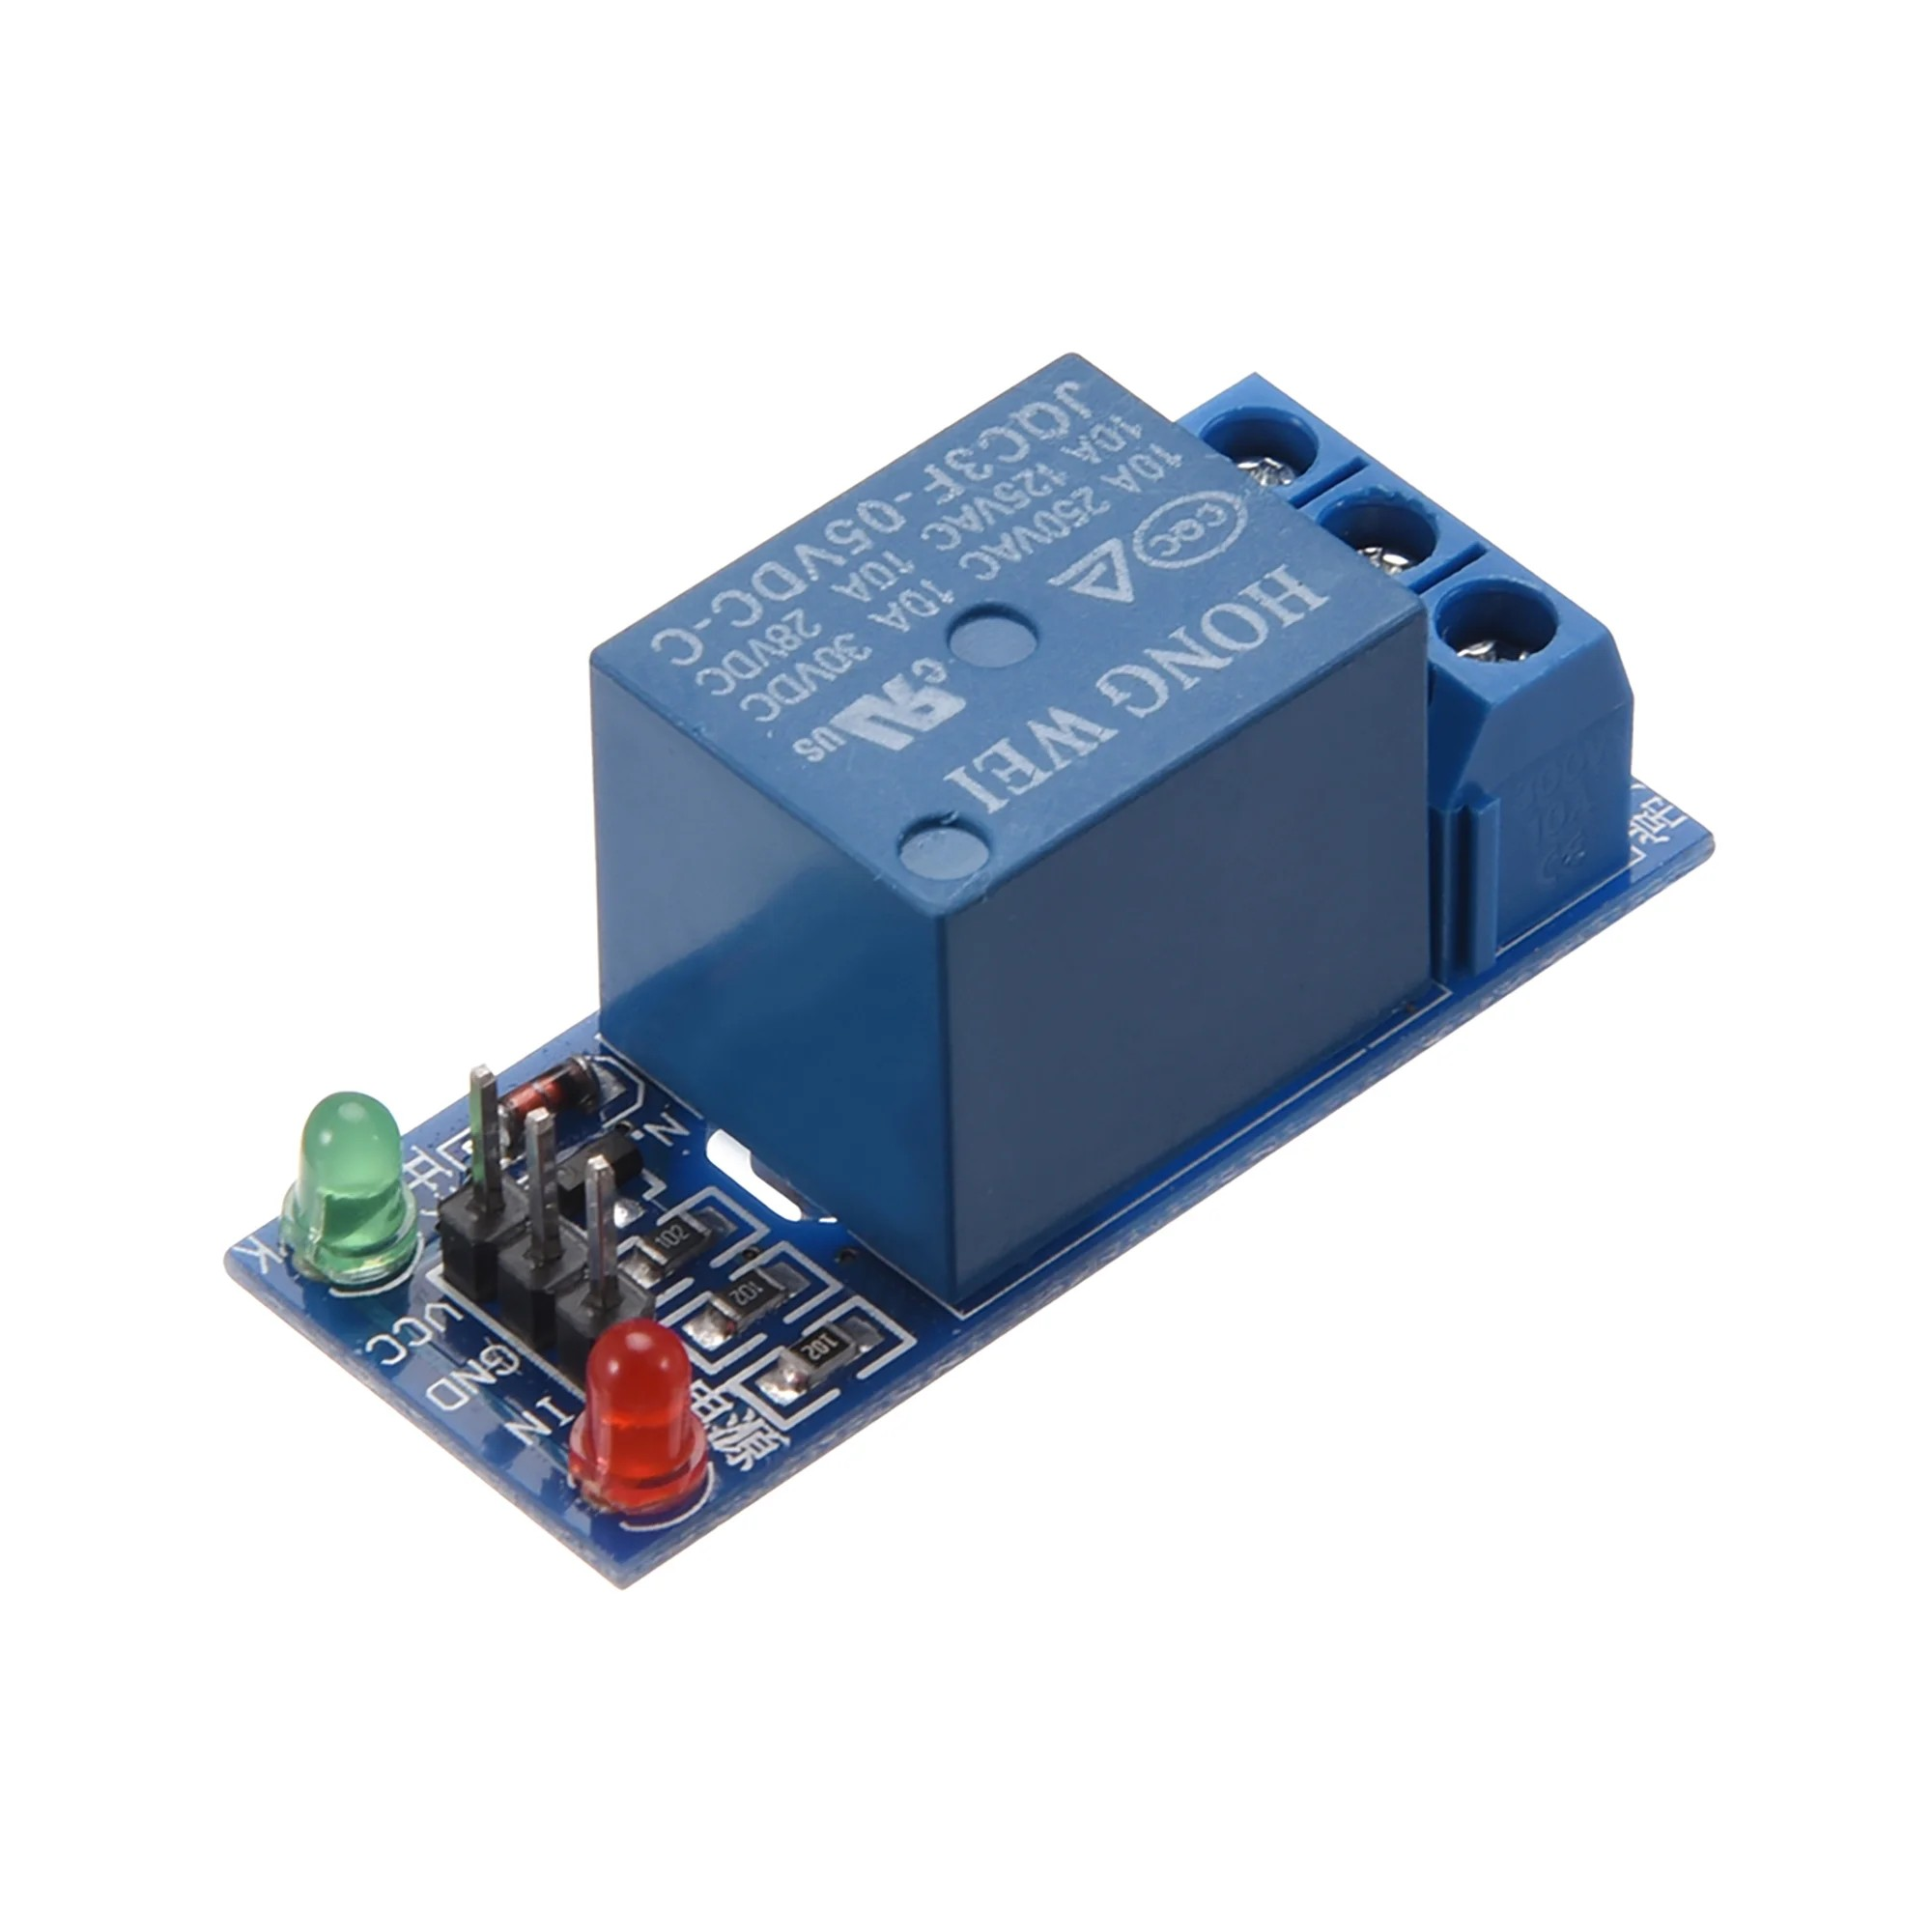
\includegraphics[width=0.8\textwidth]{Relay.jpg}
			\caption{Relay Module}
		\end{subfigure}
		\hfill
		\begin{subfigure}{0.3\textwidth}
			\centering
			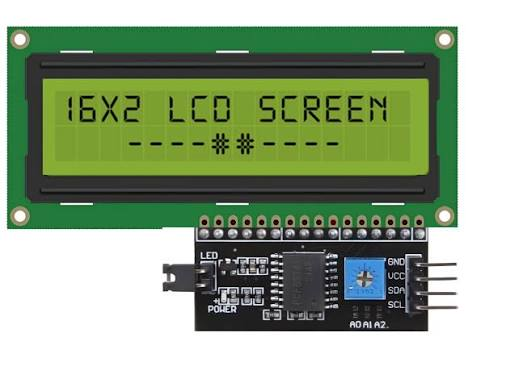
\includegraphics[width=0.8\textwidth]{LCD.jpg}
			\caption{I2C LCD Display}
		\end{subfigure}
		\hfill
		\begin{subfigure}{0.3\textwidth}
			\centering
			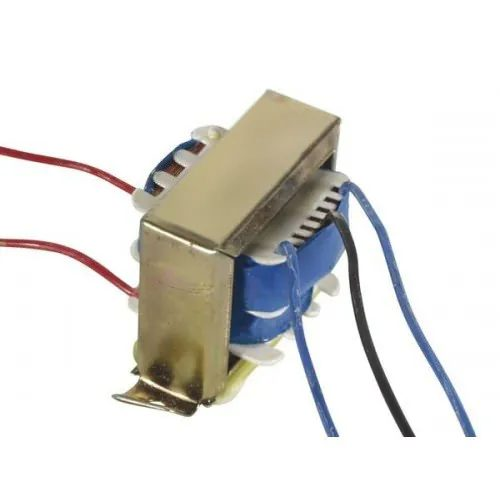
\includegraphics[width=0.8\textwidth]{Transformer.jpg}
			\caption{Step-down Transformer}
		\end{subfigure}
		
		\caption{Primary hardware components utilized in the protective relay prototype.}
	\end{figure}
	
	\begin{itemize}
		\item \textbf{Microcontroller (Arduino Uno):} The brain of the system, responsible for sampling the current, computing the IEC equation, and executing trip logic.
		\item \textbf{Current Sensing Unit:} Utilizing the ZMCT103C micro precision current transformer and PZEM-004T module to safely step down and measure the AC load current.
		\item \textbf{Isolation and Tripping (Relay Module):} A 1-channel 5V relay acts as the circuit breaker, physically disconnecting the load when a trip signal is issued.
		\item \textbf{Human-Machine Interface (HMI):} An I2C 16x2 LCD displays the real-time RMS current, calculated trip time, and system status. Push buttons are used to increment/decrement the $TMS$ and $I_s$ values. A buzzer provides an audible alarm upon tripping.
		\item \textbf{Test Load:} High-power wire-wound resistors are used to simulate varying load and fault conditions.
	\end{itemize}
	
	\newpage
	% ---------------- SECTION 3: SYSTEM ARCHITECTURE ---------------- %
	\section{System Architecture and Methodology}
	
		\subsection{Current Sampling and Signal Processing}
	The continuous AC current from the main line is stepped down by the current transformer. Because the Arduino's Analog-to-Digital Converter (ADC) operates strictly in the positive voltage domain (0 to 5V), the bipolar AC signal is DC-biased (offset to 2.5V). 
	
	The microcontroller samples this analog signal at a high frequency. The control algorithm calculates the True RMS value by subtracting the DC offset, squaring the discrete samples, computing the mean over a full 50 Hz AC cycle (20 ms), and finally taking the square root. This robust digital signal processing ensures high immunity to harmonics and noise, which is critical for accurate fault detection.
	
	\subsection{Inverse-Time Control Algorithm}
	The core logic relies on accurately executing the IEC Very Inverse characteristic. Once the calculated RMS current exceeds the user-defined pickup current ($I_s$), the microcontroller enters the fault-handling routine. The target tripping time ($t_{trip}$) is computed dynamically using Equation 1 based on the instantaneous Plug Setting Multiplier ($PSM$).
	
	To handle transient or self-clearing faults, the control algorithm employs an active execution timer. If the current remains above $I_s$, the timer increments. If the current drops below the pickup value before the timer reaches $t_{trip}$, the fault is considered transient, and the timer resets to zero, preventing nuisance tripping. If the timer reaches or exceeds $t_{trip}$, the microcontroller instantly sends a HIGH logical signal to the relay module, opening the circuit, while activating the buzzer and displaying a "FAULT" message on the LCD.
	
	\subsection{Block Diagram}
	The hardware architecture follows a standard closed-loop protective relay design. As shown in Figure 2, the AC current passes through the test load and is monitored by the Current Sensor. The analog signal is fed into the Microcontroller. Based on the HMI settings (Push Buttons) and the internal logic, the Microcontroller dictates the state of the Trip Relay and updates the LCD/Buzzer.
	
	\begin{figure}[H]
		\centering
		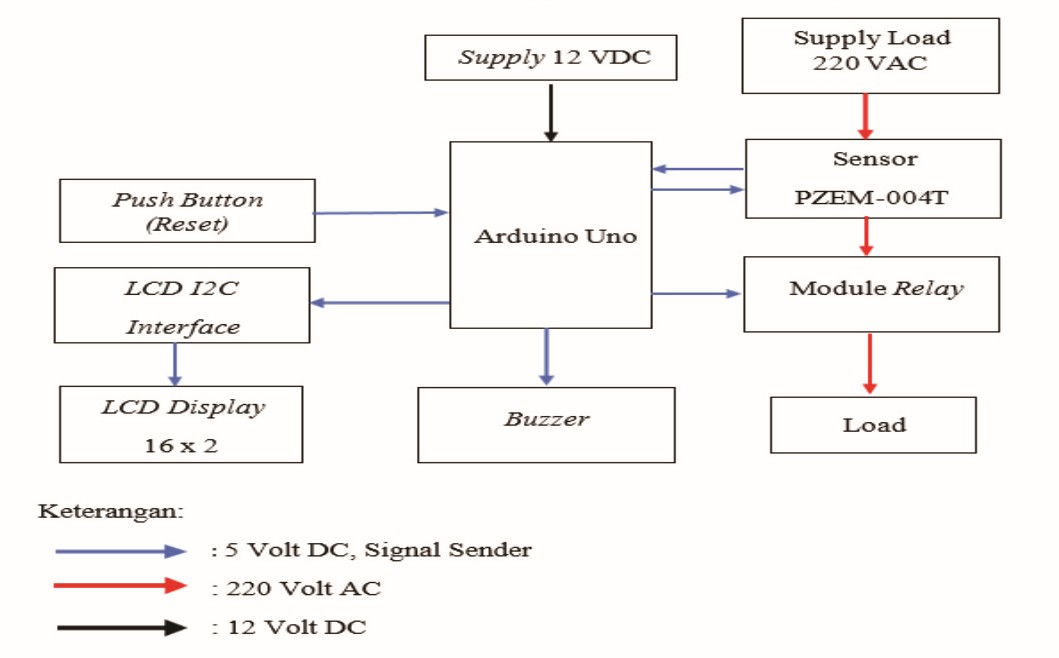
\includegraphics[width=0.6\textwidth]{block_diagram.jpg}
		\caption{Block Diagram of the Microcontroller-Based Overcurrent Relay.}
	\end{figure}
	
	\newpage
	\subsection{Software Flowchart}
	The software logic is designed for continuous, non-blocking monitoring. Figure 3 details the execution flow. The program continuously reads the RMS current and compares it against the Pickup Current ($I_s$). 
	
	If $I < I_s$, the system remains in normal operation, and the LCD displays the current. If $I \geq I_s$, a fault is detected. The microcontroller immediately calculates the required trip time using the Very Inverse formula. An internal timer starts; if the fault persists for the calculated duration, the trip signal is activated, the load is disconnected, and the buzzer sounds.
	
	\begin{figure}[H]
		\centering
		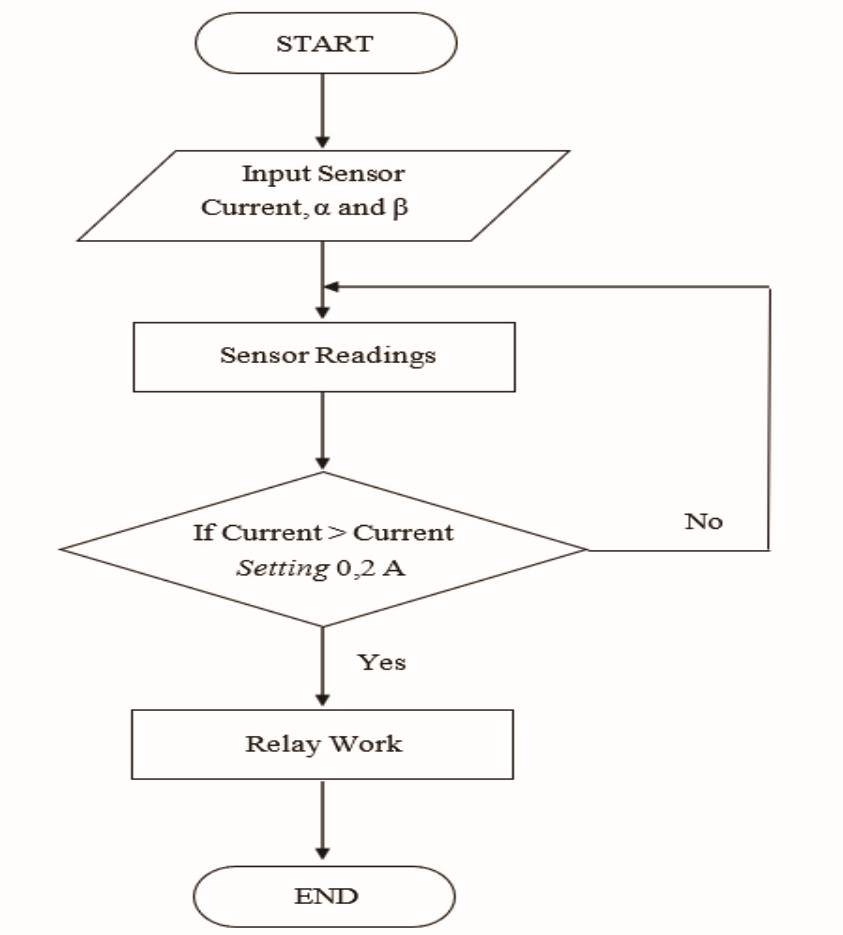
\includegraphics[width=0.55\textwidth]{flowchart.jpg}
		\caption{Software Execution Flowchart for the Inverse Time Logic.}
	\end{figure}
	
	\newpage
	% ---------------- SECTION 4: RESULTS ---------------- %
	\section{System Testing and Characteristics}
	The relay's performance was verified by subjecting it to varying fault current levels and comparing the actual tripping time with the theoretical IEC curve. 
	
	Figure 4 illustrates the Time-Current characteristic curve plotted from the system's operational data. As the Plug Setting Multiplier ($PSM = \frac{I}{I_s}$) increases, the tripping time decreases inversely. The curve confirms that the software successfully mimics an electromechanical Very Inverse relay, providing fast fault clearance for severe short circuits while allowing temporary minor overloads (beneficial for motor starting or transient inrush currents) without nuisance tripping.
	
	\begin{figure}[H]
		\centering
		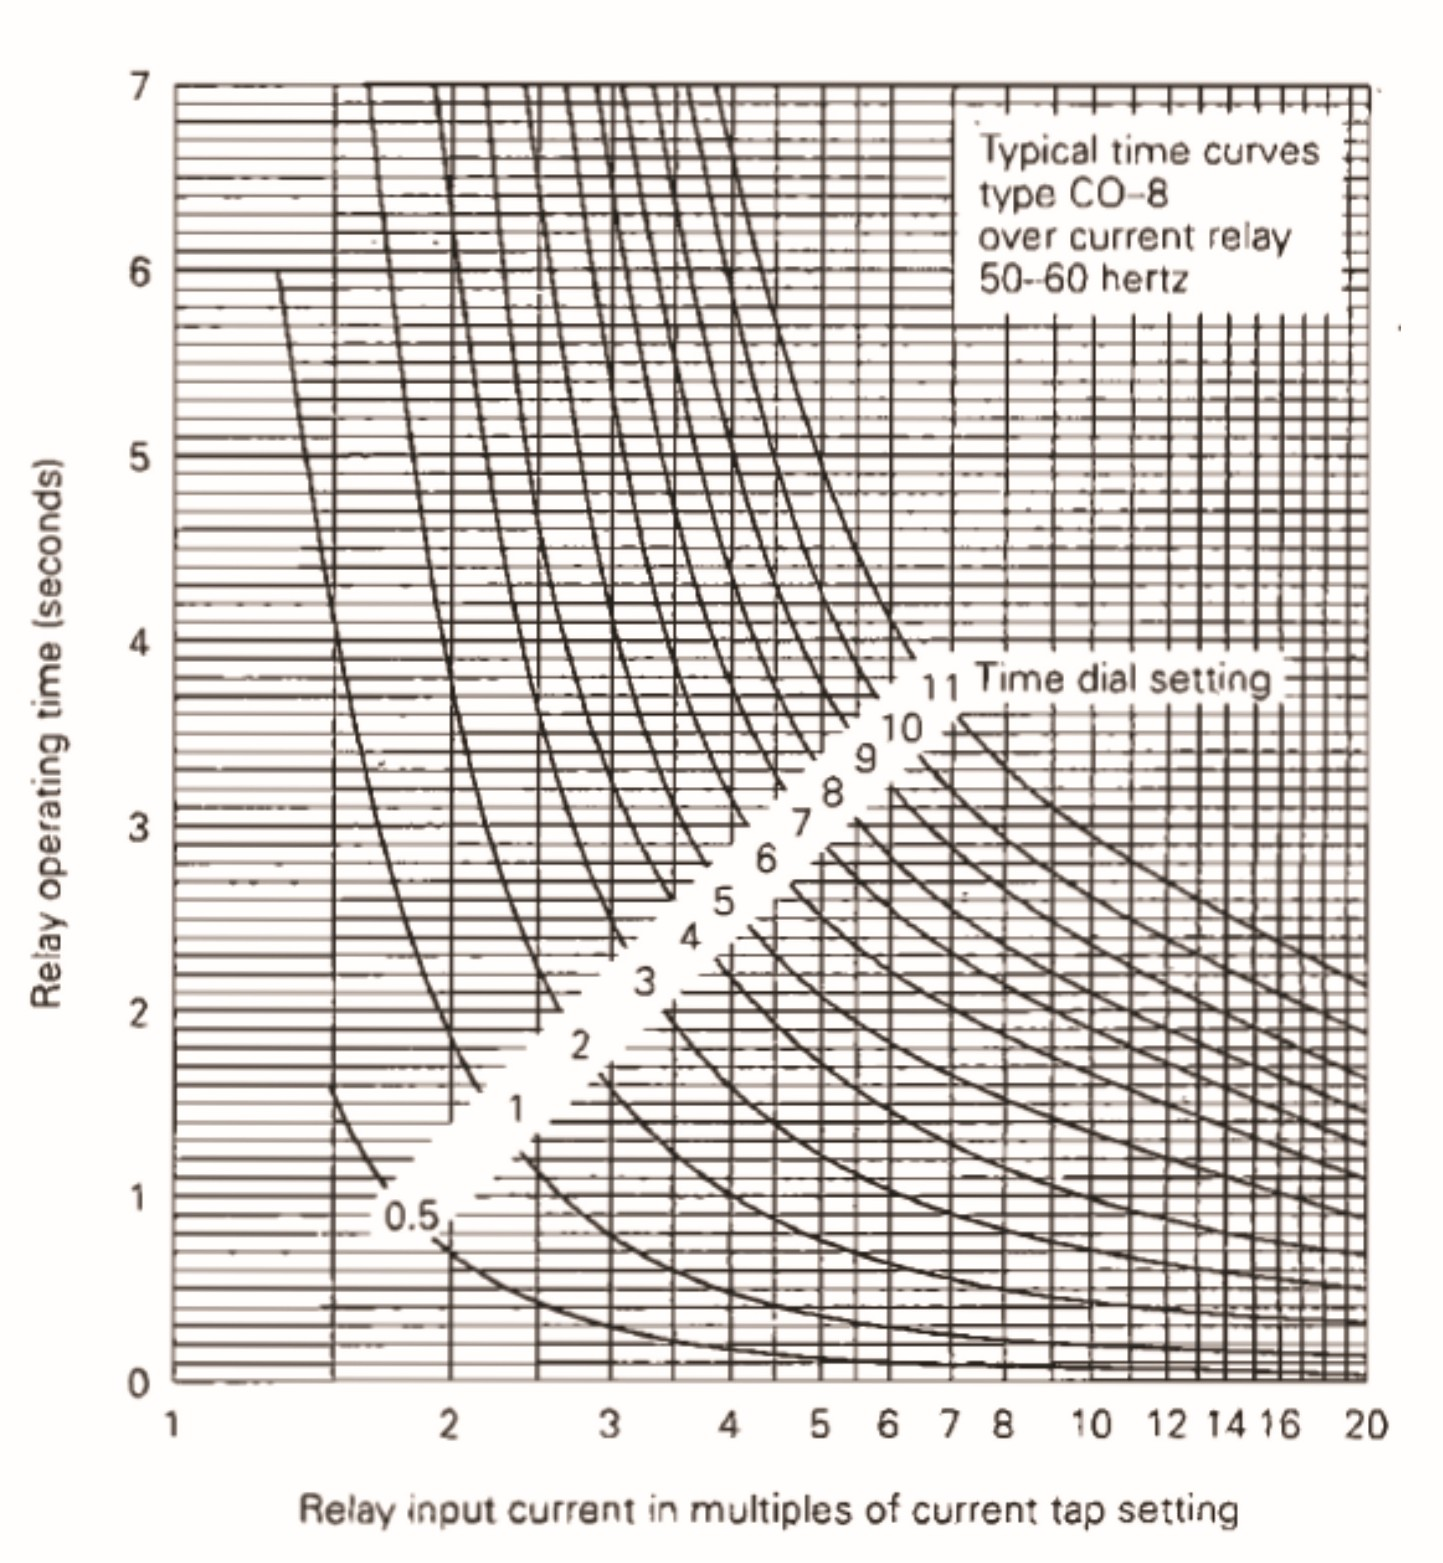
\includegraphics[width=0.85\textwidth]{time_curve.jpg}
		\caption{IEC Very Inverse Time-Current Characteristic Curve implemented in the code.}
	\end{figure}
	
	\newpage
	
	\section{Conclusion}
	This project successfully demonstrated the design and implementation of a digital overcurrent relay utilizing an Arduino microcontroller. By integrating precise current sensing components and embedding the IEC Very Inverse time-current equation into the software, the prototype effectively protected the circuit against various overcurrent scenarios. The addition of a user-friendly HMI (LCD and push buttons) allowed for dynamic adjustment of the protection parameters ($I_s$ and $TMS$), replicating the flexibility found in modern industrial numerical relays. This implementation bridges the gap between theoretical power system protection concepts and practical, low-cost embedded hardware design.
	
\end{document}